%----------------------------------------------------------------------------------------
%	SOLUTION 4.i
%----------------------------------------------------------------------------------------
\subsection*{Problem 4.i}
The time domain dynamics of the circuit is given by:
\begin{align*}
	\begin{bmatrix}
		v_t^a\\v_t^b\\v_t^c
	\end{bmatrix} &= L \frac{\text{d}}{\text{d}t}\begin{bmatrix}
		i_a\\i_b\\i_c
	\end{bmatrix} + R \begin{bmatrix}
		i_a\\i_b\\i_c
	\end{bmatrix}+\begin{bmatrix}
		v_0^a\\v_0^b\\v_0^c
	\end{bmatrix}.
\end{align*}
Converting them to d-q domain (at an angle $\theta_d=\omega_d t$) as illustrated in Q3, we get:
\begin{align*}
	&\Gamma_{dq}^T \begin{bmatrix}
		v_t^d\\v_t^q
	\end{bmatrix} = L\frac{\text{d}}{\text{d}t}\left(\Gamma_{dq}^T\begin{bmatrix}
		i_d\\i_q
	\end{bmatrix}\right)+R\Gamma_{dq}^T\begin{bmatrix}
		i_d\\i_q
	\end{bmatrix}+\Gamma_{dq}^T\begin{bmatrix}
		v_0^d\\v_0^q
	\end{bmatrix}\\
	\implies & \Gamma_{dq}^T\begin{bmatrix}
		v_t^d\\v_t^q
	\end{bmatrix} = L\dot{\theta_d}\Gamma_{dq}^T\begin{bmatrix}
		0 & -1\\1 & 0
	\end{bmatrix}\begin{bmatrix}
		i_d\\i_q
	\end{bmatrix}+L\Gamma_{dq}^T\begin{bmatrix}
		\dot{i_d}\\\dot{i_q}
	\end{bmatrix}+R\Gamma_{dq}^T\begin{bmatrix}
		i_d\\i_q
	\end{bmatrix}+\Gamma_{dq}^T\begin{bmatrix}
		v_0^d\\v_0^q
	\end{bmatrix}\\
	\implies & \begin{bmatrix}
		v_t^d\\v_t^q
	\end{bmatrix} = L\omega_d\begin{bmatrix}
		-i_q\\i_d
	\end{bmatrix}+L\begin{bmatrix}
		\dot{i_d}\\\dot{i_q}
	\end{bmatrix}+R\begin{bmatrix}
		i_d\\i_q
	\end{bmatrix}+\begin{bmatrix}
		v_0^d\\v_0^q
	\end{bmatrix}.
\end{align*}
Converting the above equations in block diagrams along with feedback control and following Fig.~3 in the question for point of feed forward, we get the following block diagram shown in Fig.~\ref{fig:q4_block_dia} in dq domain as requested in the question.
%%%%%%%%%%%%%%%%%%%%%%% BLOCK DIAGRAM %%%%%%%%%%%%%%%%%%%%%
\begin{figure}[!h]
	\centering
	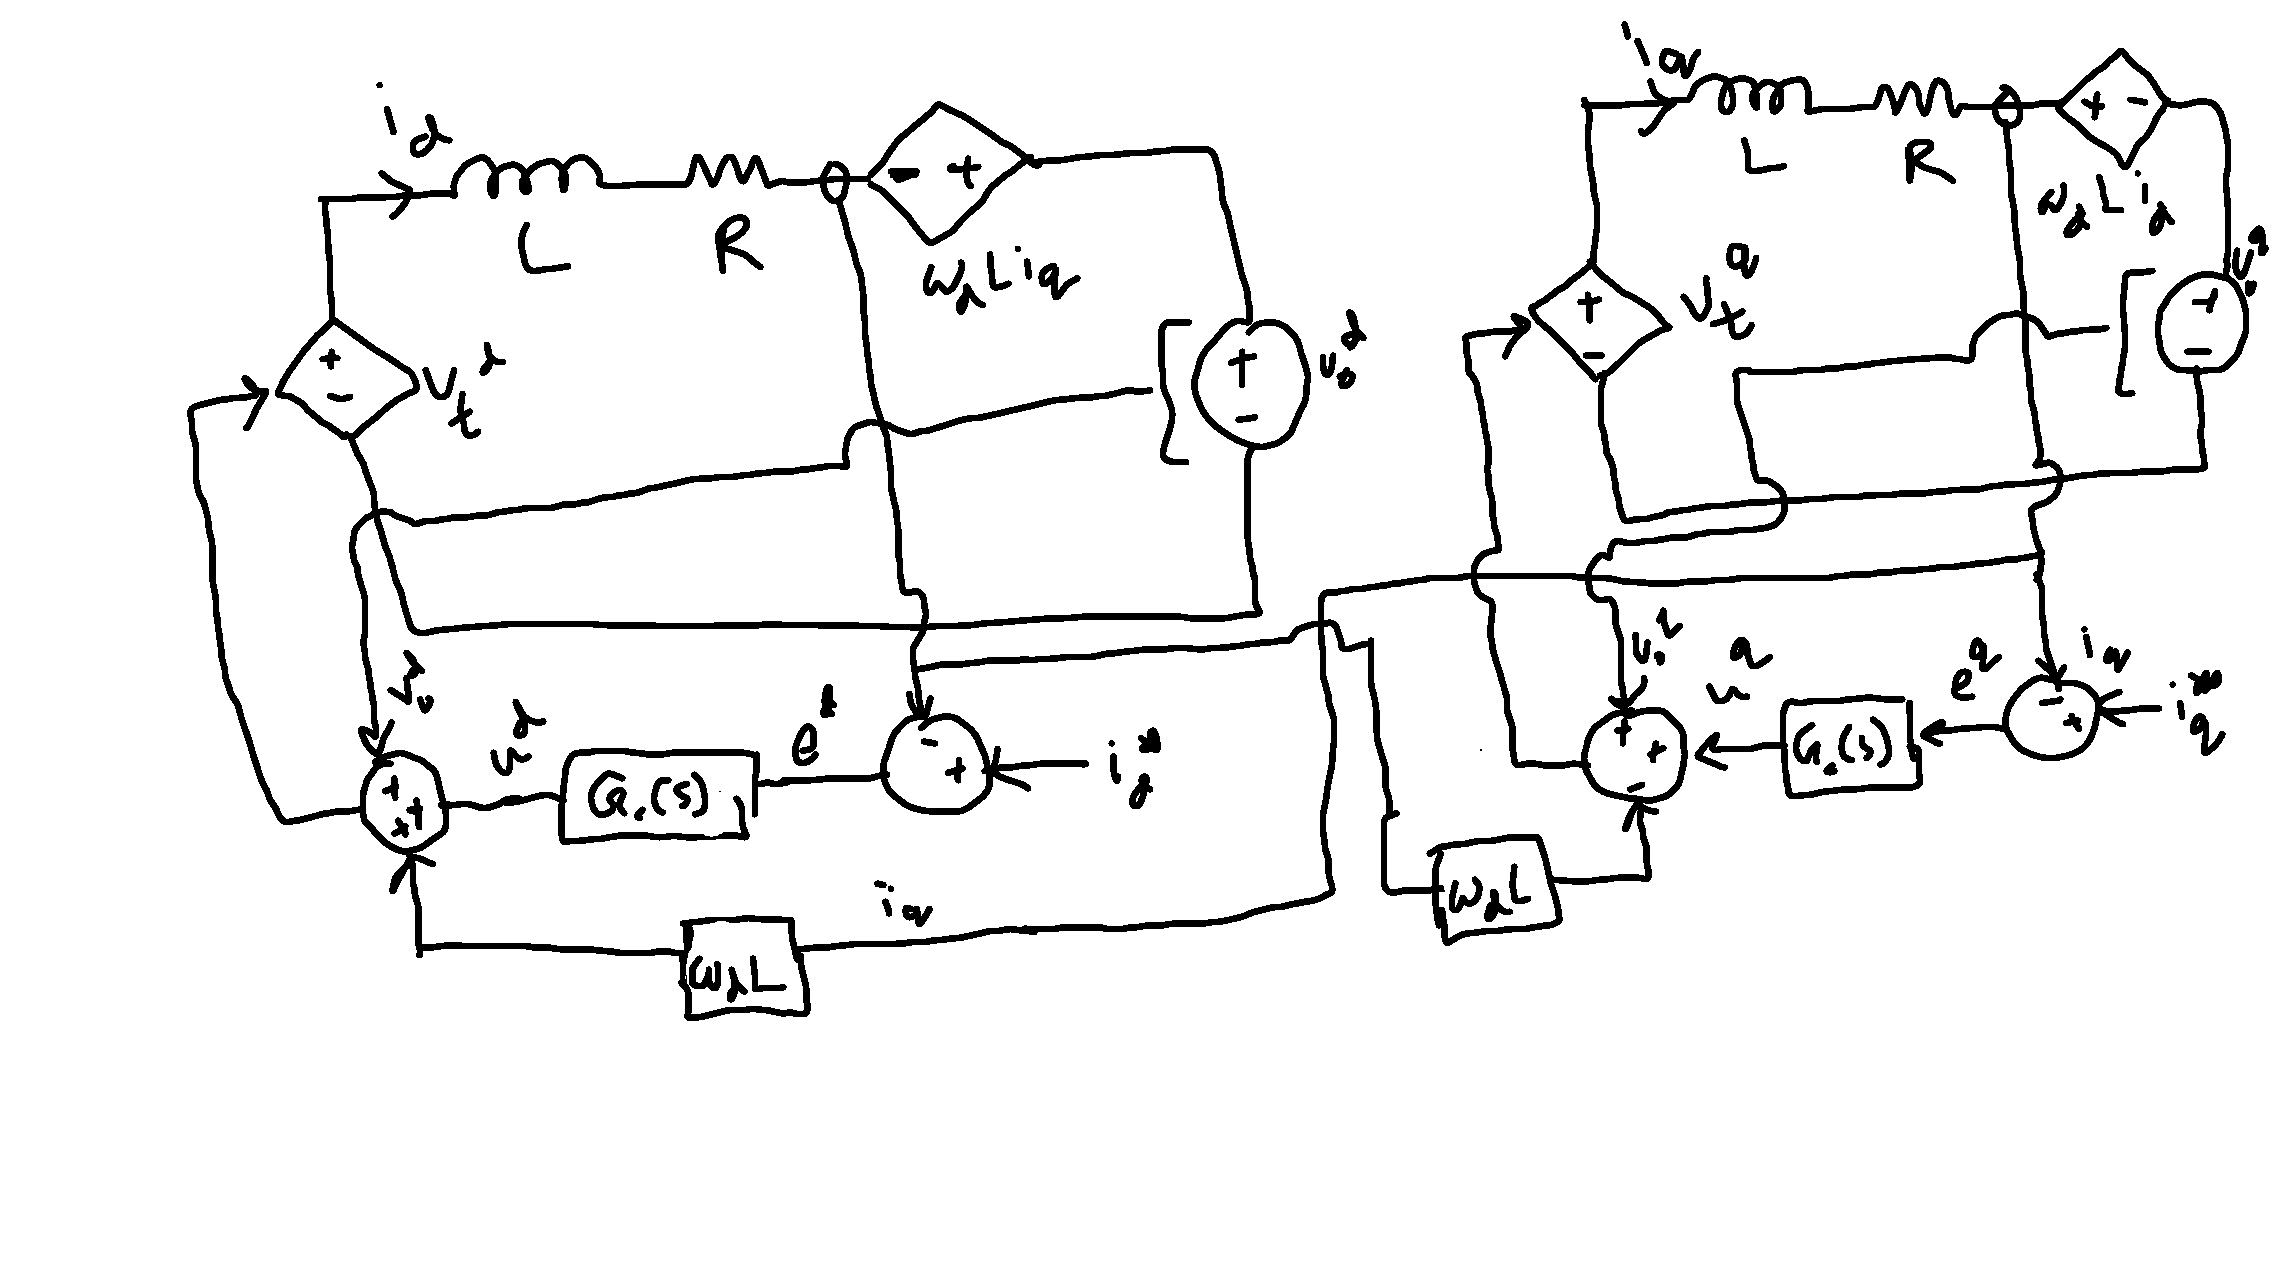
\includegraphics[scale=0.4,trim={2cm 4cm 0cm 0cm},clip]{q4_block_dia.pdf}
	\caption{Q4: Inverter feedback control block diagram}
	\label{fig:q4_block_dia}
\end{figure}
%----------------------------------------------------------------------------------------
%	SOLUTION 4.ii
%----------------------------------------------------------------------------------------
\subsection*{Problem 4.ii}
To derive the closed-loop transfer functions $\frac{i_{dq}(s)}{i_{dq}^*(s)}$, we need to ignore the cross-coupling terms and $v_{dc}$ in Fig.~3 (in the question). Then we can get the following the block diagram for $i_d(s)$ (similar diagram for $i_q(s)$ too) as shown in Fig.~\ref{fig:q4_tf}:
%%%%%%%%%%%%%%%%%%%%%%% TRANSFER FUNCTION %%%%%%%%%%%%%%%%%%%%%
\begin{figure}[!h]
	\centering
	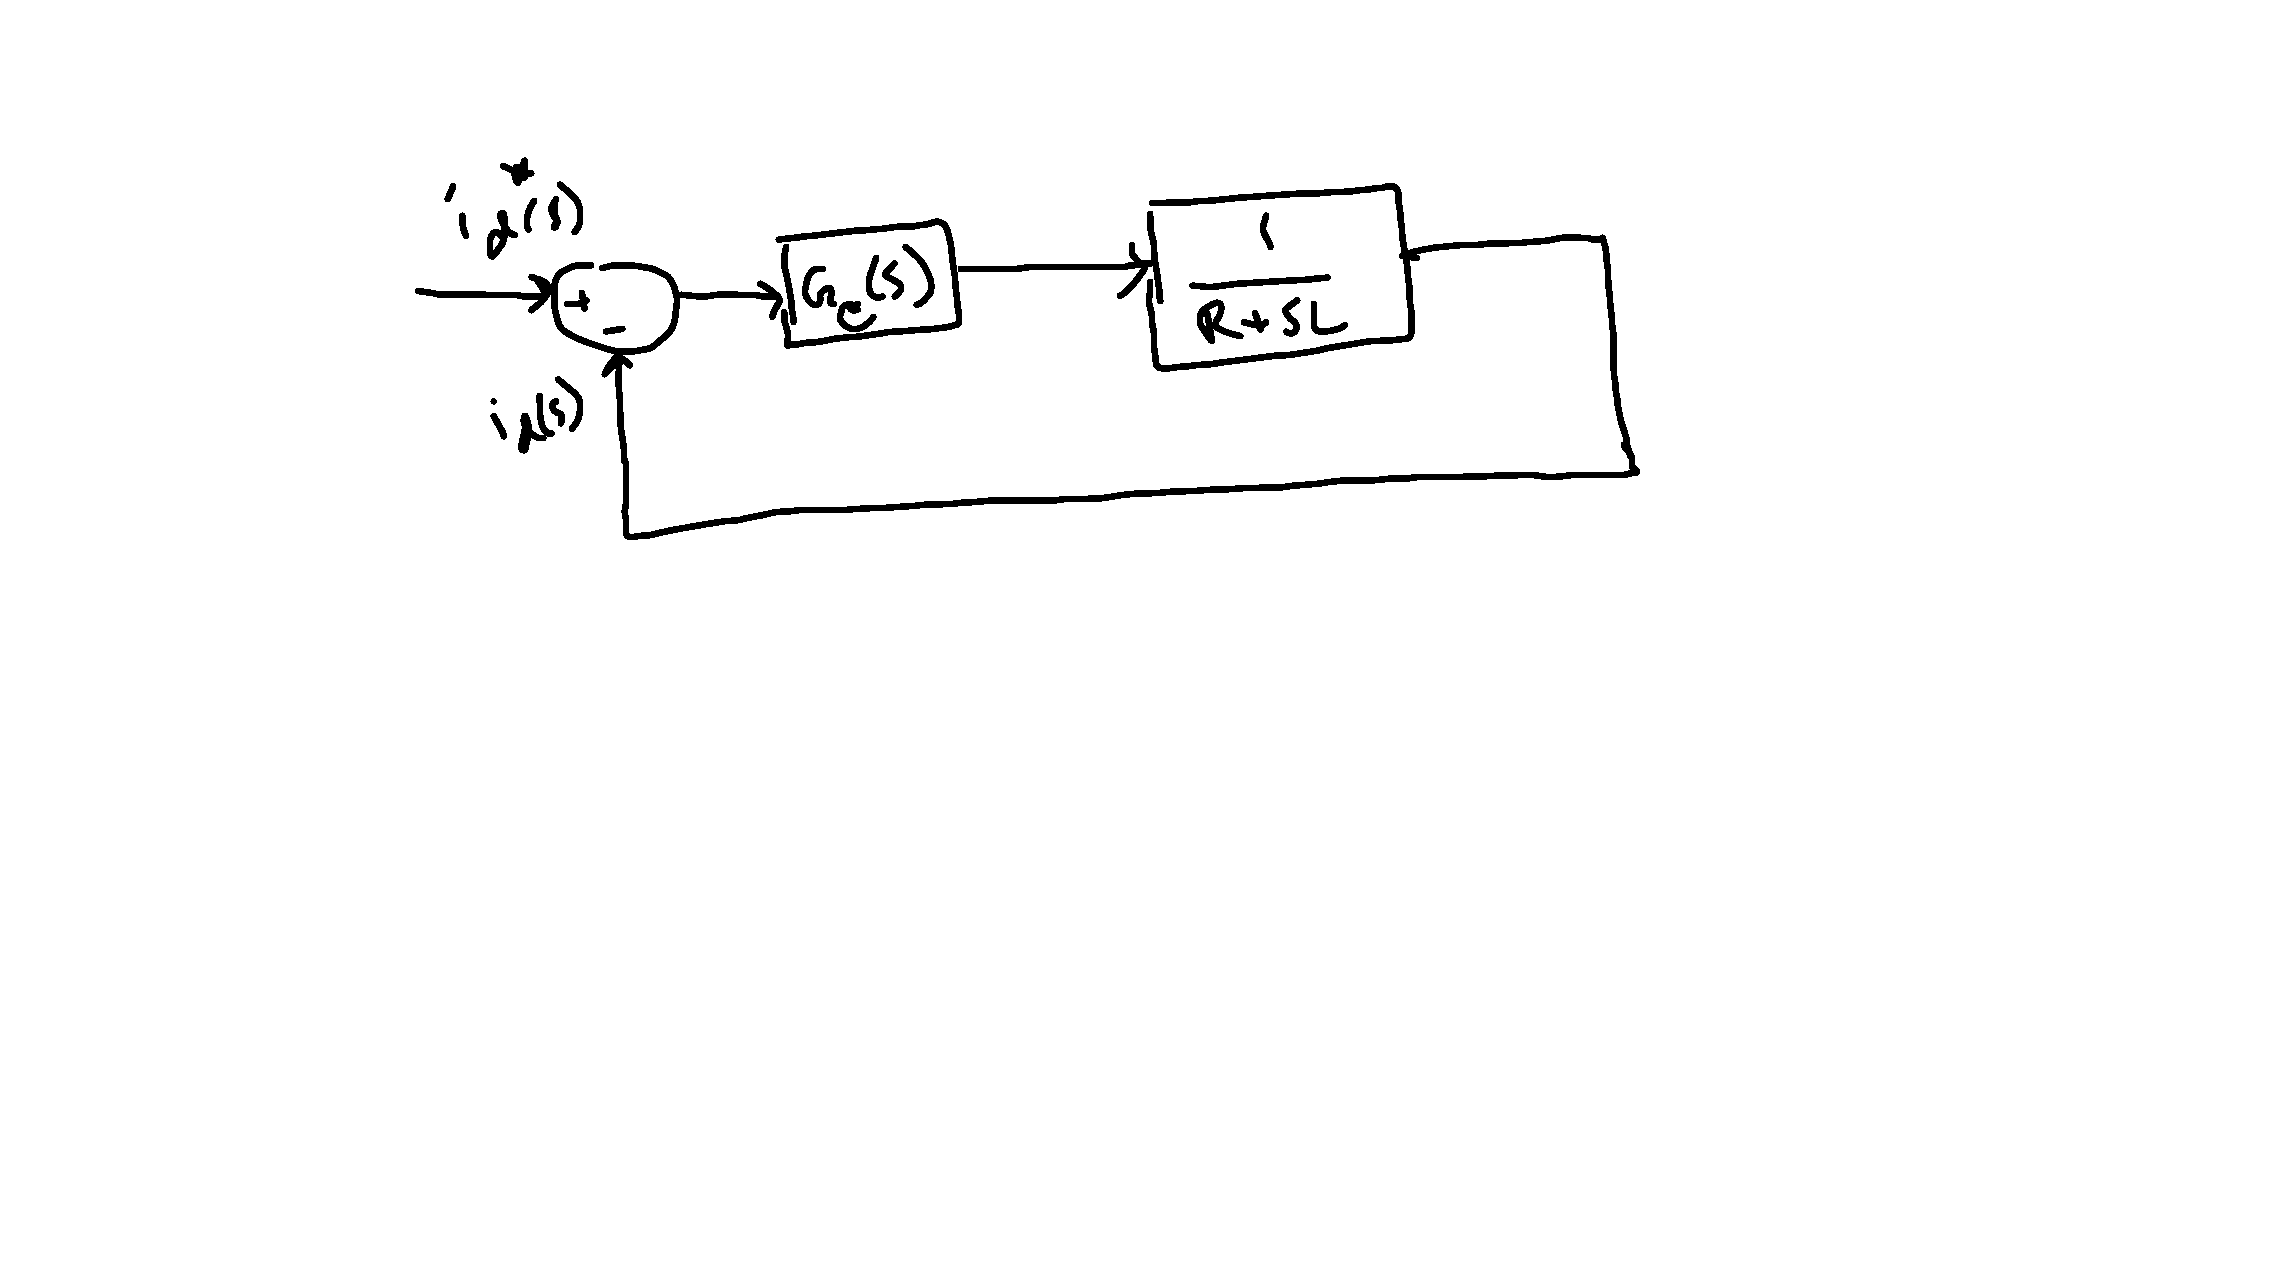
\includegraphics[scale=0.4,trim={2cm 12cm 0cm 0cm},clip]{q4_tf.pdf}
	\caption{Q4: Block diagram to derive current transfer function}
	\label{fig:q4_tf}
\end{figure}

Considering $G_c(s)=(k_p+k_i/s)$, we can derive the transfer function as follows:
\begin{align}\label{eq:q4_tf}
	H(s) &= \frac{i_d(s)}{i_d^*(s)} \nonumber\\
	&= \frac{G_c(s)/(R+sL)}{1+G_c/(R+sL)} \nonumber\\
	&= \frac{G_c(s)}{(R+sL)+G_c(s)} \nonumber\\
	&= \frac{k_p+k_i/s}{(k_p+k_i/s)+(R+sL)}.
\end{align}
%----------------------------------------------------------------------------------------
%	SOLUTION 4.iii
%----------------------------------------------------------------------------------------
\subsection*{Problem 4.iii}
From Eq.~\ref{eq:q4_tf}, we get,
\begin{align}\label{eq:q4_iii_a}
	H(s) &= \frac{sk_p+k_i}{s^2L+s(R+k_p)+k_i} \nonumber\\
	&= \frac{1}{\frac{s^2L}{sk_p+k_i}+\frac{s(R+k_p)}{sk_p+k_i}+\frac{k_i}{sk_p+k_i}}
\end{align}
Equating denominator of Eq.~\ref{eq:q4_iii_a} with that of desired transfer function $\frac{1}{1+\tau s}$, we get:
\begin{align*}
	&\frac{s^2L}{sk_p+k_i}+\frac{s(R+k_p)}{sk_p+k_i}+\frac{k_i}{sk_p+k_i} = (1+\tau s)\\
	\implies & s^2L+s(R+k_p)+k_i = s^2 \tau k_p + s(k_p+\tau k_i)+k_i.
\end{align*}
Equating corresponding coefficients of $s$, we get:
\begin{align*}
	L &= \tau k_p \implies \tau = \frac{L}{k_p}\\
	R+k_p &= k_p+\tau k_i \implies \tau = \frac{R}{k_i}.
\end{align*}
Therefore,
\begin{align*}
	&\frac{L}{k_p} = \frac{R}{k_i}\\
	\implies & \frac{L}{R} = \frac{k_p}{k_i}.
\end{align*}
Similarly, we can prove the \textit{only if} part as follows.\\
Let, $\frac{L}{R}=\frac{k_p}{k_i}=c$. Also denote $\tau \coloneqq \frac{R}{k_i}$. Then $\tau = \frac{L}{k_p}$ also. From Eq.~\ref{eq:q4_tf},
\begin{align*}
	H(s) &= \frac{k_p+k_i/s}{(k_p+k_i/s)+(R+sL)}\\
	&= \frac{1}{1+\frac{R+sL}{k_p+k_i/s}}\\
	&= \frac{1}{1+\frac{(R/k_i)+s(L/k_i)}{(k_p/k_i)+(1/s)}}\\
	&= \frac{1}{1+\frac{\tau+s\frac{L}{k_p}\frac{k_p}{k_i}}{c+(1/s)}}\\
	&= \frac{1}{1+\frac{\tau + sc\frac{L}{k_p}}{c+(1/s)}}\\
	&= \frac{1}{1+\frac{s\tau+s^2c\tau}{sc+1}}\\
	&= \frac{1}{1+\tau s}.
\end{align*}
